\newcommand*{\ImplementationPath}{04-framework/02-implementation}

The break-down in Section \ref{sec:design} can be implemented in any number of ways. 
This section focuses on its implementation details and is divided into four parts following the organization presented in Figure \ref{fig:framework-design}: database overview, sentiment analysis APIs and script collection and web server overview. 
Since choices made in either of those parts regarding structure and technology are mutually depended, here we'll define the technologies used in order to make the sections which follow more intelligible:
\begin{description}
\singlespacing
 \item[DBMS:] MySQL 5.5.3+
 \item[Web framework:] Django 1.9 
 \item[Sentiment analysis scripts:] python 2.7.+
\end{description}

% --- SECTION DATABASE OVERVIEW---
\newcommand*{\DatabaseOverviewPath}{04-framework/02-implementation/01-database}

% --- SUBSECTION DATABASE ---
\subsection{Database overview\label{sec:database-overview}}
All the data acquired or generated is stored in a single relational database called \inlinecode{sentiment\_db}. 
The logical view of the database is shown in Figure \ref{fig:db-schema}. 
In favor of clarity parts considered inconsequential to sentiment analysis processes are not disclosed. 
Those include, but are not limited to: django sessions, brands etc.
\usetikzlibrary{positioning,shapes,arrows}

\tikzstyle{table}=[rectangle, rectangle split, rectangle split parts=2, rounded corners=2pt, draw=black,fill=white, inner sep=0.2cm, font=\scriptsize\mdseries]
\tikzstyle{line}=[>-, thick, dashed]
        
\begin{figure}[H]
\centering  
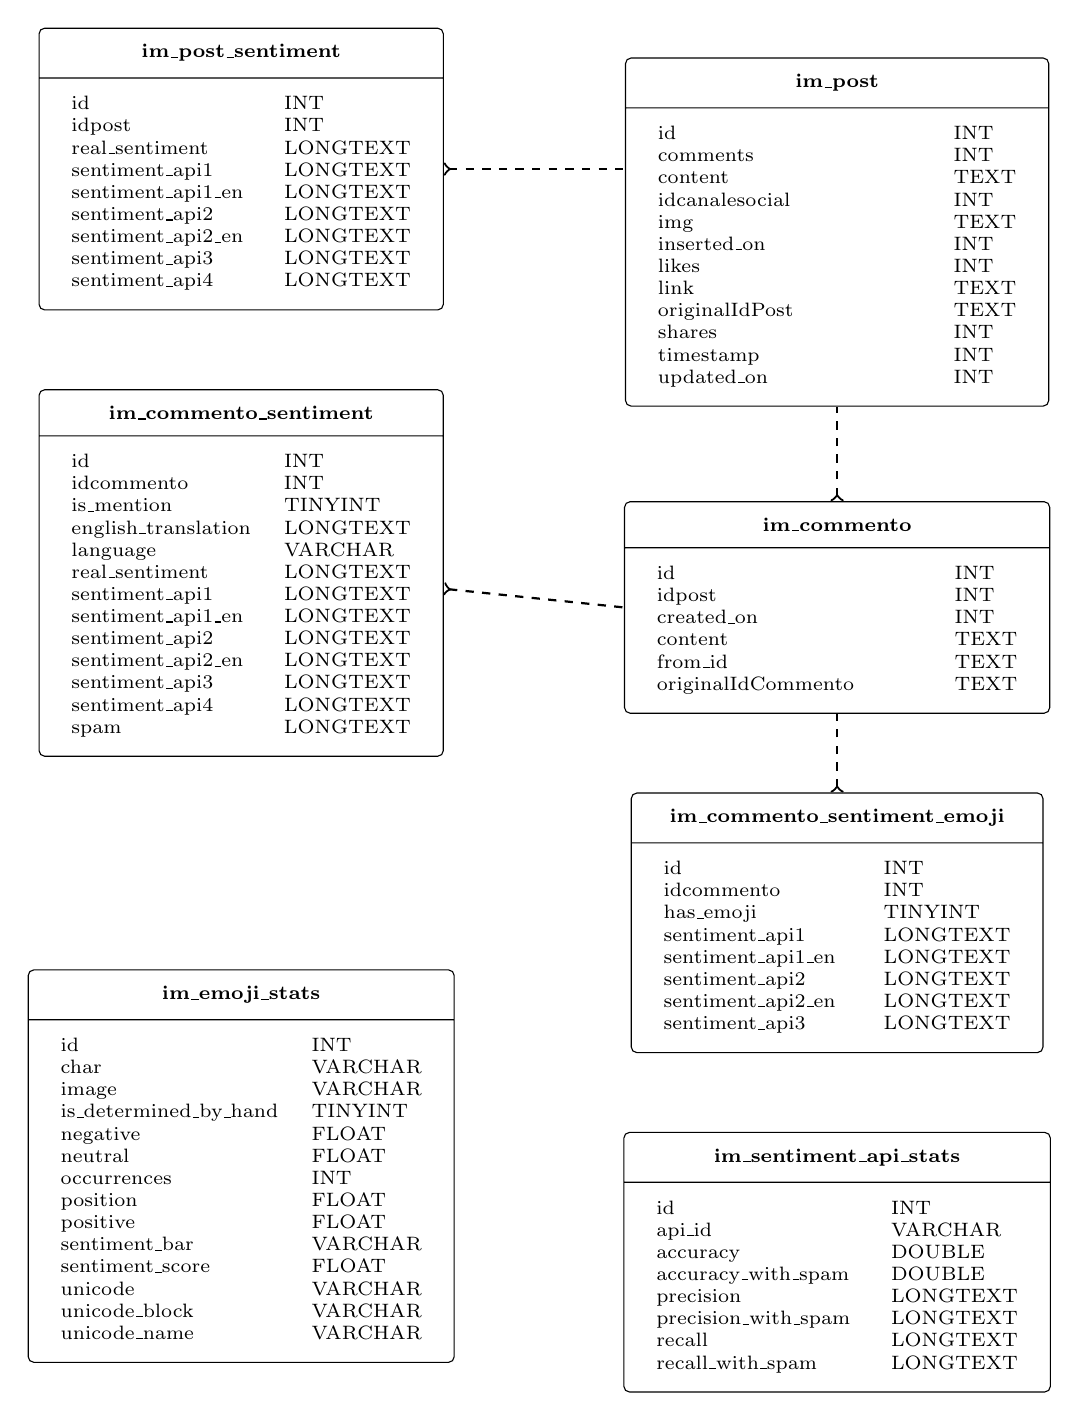
\begin{tikzpicture}[node distance=1cm]
\onehalfspacing

    \node (im-post) [table]{
        \textbf{im\_post}
        \nodepart{second}
            \tabular{ll} 
            id & INT \\ 
            comments & INT \\ 
            content & TEXT \\ 
            idcanalesocial & INT \\ 
            img & TEXT \\ 
            inserted\_on & INT \\ 
            likes & INT \\ 
            link & TEXT \\ 
            originalIdPost \ \ \ \ \ \ \ \ \ \ \ \ \ \ \ \ \ & TEXT \\
            shares & INT \\
            timestamp & INT \\
            updated\_on & INT \\                        
            \endtabular
    };

    \node (im-post-sentiment) [table, left=of im-post, yshift=0.8cm, xshift=-1.3cm]{
        \textbf{im\_post\_sentiment}
        \nodepart{second}
            \tabular{ll}                    
            id & INT \\
            idpost & INT \\
            real\_sentiment & LONGTEXT \\
            sentiment\_api1 & LONGTEXT \\
            sentiment\_api1\_en \ & LONGTEXT \\
            sentiment\_api2 & LONGTEXT \\
            sentiment\_api2\_en & LONGTEXT \\
            sentiment\_api3 & LONGTEXT \\
            sentiment\_api4 & LONGTEXT \\
            \endtabular
    };

    \node (im-commento) [table, below=of im-post,yshift=-0.2cm ]{
        \textbf{im\_commento}
        \nodepart{second}
            \tabular{ll}                    
            id & INT \\
            idpost & INT \\
            created\_on & INT \\
            content & TEXT \\
            from\_id & TEXT \\
            originalIdCommento \ \ \ \ \ \ \ \ \ & TEXT \\
            \endtabular
    };

    \node (im-commento-sentiment) [table, below=of im-post-sentiment]{
        \textbf{im\_commento\_sentiment}
        \nodepart{second}
            \tabular{ll}                    
            id & INT \\
            idcommento & INT \\
            is\_mention & TINYINT \\
            english\_translation & LONGTEXT \\
            language & VARCHAR \\
            real\_sentiment & LONGTEXT \\
            sentiment\_api1 & LONGTEXT \\
            sentiment\_api1\_en & LONGTEXT \\
            sentiment\_api2 & LONGTEXT \\
            sentiment\_api2\_en & LONGTEXT \\
            sentiment\_api3 & LONGTEXT \\
            sentiment\_api4 & LONGTEXT \\
            spam & LONGTEXT \\
            \endtabular
    };

    \node (im-commento-sentiment-emoji) [table, below=of im-commento]{
        \textbf{im\_commento\_sentiment\_emoji}
        \nodepart{second}
            \tabular{ll}                    
            id & INT \\
            idcommento & INT \\
            has\_emoji & TINYINT \\
            sentiment\_api1 & LONGTEXT \\
            sentiment\_api1\_en & LONGTEXT \\
            sentiment\_api2 & LONGTEXT \\
            sentiment\_api2\_en  \ \ & LONGTEXT \\
            sentiment\_api3 & LONGTEXT \\
            \endtabular
    };

    \node (im-sentiment-api-stats) [table, below=of im-commento-sentiment-emoji]{
        \textbf{im\_sentiment\_api\_stats}
        \nodepart{second}
            \tabular{ll}                    
            id & INT \\
            api\_id & VARCHAR \\
            accuracy & DOUBLE \\
            accuracy\_with\_spam & DOUBLE \\
            precision & LONGTEXT \\
            precision\_with\_spam \ & LONGTEXT \\
            recall & LONGTEXT \\
            recall\_with\_spam & LONGTEXT \\
            \endtabular
    };

    \node (im-emoji-stats) [table, below=of im-commento-sentiment, yshift=-1.7cm]{
        \textbf{im\_emoji\_stats}
        \nodepart{second}
            \tabular{ll}                    
            id & INT \\
            char & VARCHAR \\
            image & VARCHAR \\
            is\_determined\_by\_hand & TINYINT \\
            negative & FLOAT \\
            neutral & FLOAT \\
            occurrences & INT \\
            position & FLOAT \\
            positive & FLOAT \\
            sentiment\_bar & VARCHAR \\
            sentiment\_score & FLOAT \\
            unicode & VARCHAR \\
            unicode\_block & VARCHAR \\
            unicode\_name & VARCHAR \\
            \endtabular
    };

    \draw[line] (im-post-sentiment.east) -- ([yshift=0.8cm] im-post.west);
    \draw[line] (im-commento.north) -- (im-post.south);
    \draw[line] ([yshift=-0.2cm] im-commento-sentiment.east) -- (im-commento.west);
    \draw[line] ( im-commento-sentiment-emoji.north) |- (im-commento.south);
   
\end{tikzpicture}
  \caption{Database schema}
  \label{fig:db-schema}
\end{figure}

As previously stated, we have extended and built our framework on top of a preexisting relational MySQL database schema which came with a set of specifications which were adopted and applied to \inlinecode{sentiment\_db}.
Using a version of MySQL greater or equal to 5.5.3 was a hard constraint because in that release MySQL introduced support for \inlinecode{uft8mb4} encoding.  
As opposed to \inlinecode{uft8}'s three bytes per character maximum, 
\inlinecode{uft8mb4} uses a maximum of four bytes per character making it fully compatible with \inlinecode{uft8} and, most importantly, able to correctly encode and store emojis.
It is worth mentioning that only two data tables that were a part of the original database were used and those are \inlinecode{im\_commento} and \inlinecode{im\_post}.

For the sake of completeness, following tables contain details and field descriptions of used data tables. 

\begin{table}[H]
\centering
\onehalfspacing

\begin{tabularx}{0.95\textwidth}{ l || c | X }
	\hline
	\multicolumn{3}{l}{ \textbf{im\_post} } \\
	\hline

 	\textbf{id} & INT & PRIMARY KEY \\  
	comments & INT & number of comments the post has \\  
	content & TEXT & post's content \\  
	idcanalesocial & INT & FORGEIN KEY to im\_canalesocial: \newline field links to the post's social media account \\  
	img & TEXT & url to post's accompanying photo \\  
	inserted\_on & INT & timestamp when the record was inserted \\  
	likes & INT & number of likes the post has \\  
	link & TEXT & url to the post on a social media site \\  
	originalIdPost \ \  & TEXT & identifier used on its social media site \\ 
	shares & INT & number of shares the post has \\ 
	timestamp & INT & timestamp when the post was created \\ 
	updated\_on & INT & timestamp when the record was updated \\ 
  
	\hline
\end{tabularx}
\caption{Overview of \inlinecode{im\_post} database table}
\label{tab:im-post}

\end{table}
\begin{table}[H]
\centering
\onehalfspacing

\begin{tabularx}{0.95\textwidth}{ l || c | X }
	\hline
	\multicolumn{3}{l}{ \textbf{im\_commento} } \\
	\hline

 	\textbf{id} & INT & PRIMARY KEY \\  
	idpost & INT & FORGEIN KEY to im\_post: \newline field links to the comment's post \\  
	created\_on & INT & timestamp when the comment was created \\
	content & TEXT & comment's content \\
	from\_id & TEXT & commentator's id \\
	originalIdCommento & TEXT & identifier used on its social media site \\
 
	\hline
\end{tabularx}

\caption{Overview of \inlinecode{im\_commento} database table}
\label{tab:im-commento}

\end{table}
\newpage

As mentioned, emojis play a big role in determining sentiment of a comment. 
Since none of the APIs took them into account, we used sentiment scores from \emph{Emoji Sentiment Ranking}\footnote{http://kt.ijs.si/data/Emoji\_sentiment\_ranking} published as a part of a sentiment analysis study\cite{Kralj2015emojis},  and imported them into the database table \inlinecode{im\_emoji\_stats} whose details are shown in Table \ref{tab:im-emoji-stats}.  
However, not all emojis or emoticons that occurred in our data set were included in the study (e.g. 📘 🍾 🙂 🙄 🕶 :) :D ).
Which means they had to be manually inserted in the db. 
Their sentiment scores were determined by finding a similarly defined emoji and making the assumption that they had the same, or at least similar, sentiment. 
%All emojis that were inserted by hand are marked by a true value in  \inlinecode{is\_determined\_by\_hand} column.
For example, green book's (📗) sentiment score was used in place for the missing blue book emoji (📘). 
An example of missing inserted emojis and their similar counterparts can be found in Table \ref{tab:inserted-emoticons}
\begin{table}[H]
\centering
\onehalfspacing

\begin{tabularx}{0.95\textwidth}{ c | c | c | X }
	\hline
	\textbf{Inserted icon} & \textbf{Similar icon} & \textbf{Sentiment score} & \textbf{Unicode name} \\  
 	\hline
	📘        & 📗 & 0.491 & Blue book \\
	🙂        &  ☺ & 0.72 & Slightly smiling face \\
	🕶        & 😎 & 0.491 & Dark sunglasses \\
	:-) :) =) &  ☺ & 0.657 & Smiley face \\
	:*        & 😘 & 0.71 & Kiss face \\
	<3        & ❤  &  0.657 & Heart  \\
	\hline
\end{tabularx}

\caption{Inserted emojis into \inlinecode{im\_emoji\_stats} database table}
\label{tab:inserted-emoticons}

\end{table}
\begin{table}[H]
\centering
\onehalfspacing

\begin{tabularx}{0.95\textwidth}{ l || c | X }
	\hline
	\multicolumn{3}{l}{ \textbf{im\_emoji\_stats} } \\
	\hline
 	\textbf{id} & INT & PRIMARY KEY \\  
	char & VARCHAR &  emoji  characers \\ 
	is\_determined\_by\_hand & TINYINT & boolean variable that denotes if emoji or emoticons were added by hand or used stats from the study \emph{Emoji Sentiment Ranking} \\ 
	negative & FLOAT &  how negative is the emoji $\in [0,1]$ \\ 
	neutral & FLOAT &  how neutral is the emoji $\in [0,1]$ \\ 
	occurrences & INT & number of occurrences of the emoji in all comments in our dataset \\ 
	positive & FLOAT & how positive is the emoji $\in [0,1]$ \\ 
	sentiment\_score & FLOAT & overall sentiment score $\in [-1,1]$ \\ 
	unicode & VARCHAR & unicode codepoint of the emoji \\ 
	unicode\_block & VARCHAR & general category an emoji falls into \\ 
	unicode\_name & VARCHAR & descriptive name of the emoji \\ 
	\hline
\end{tabularx}

\caption{Overview of \inlinecode{im\_emoji\_stats} database table}
\label{tab:im-emoji-stats}

\end{table}

Tables \ref{tab:im-commento-sentiment}, \ref{tab:im-post-sentiment}, \ref{tab:im-commento-sentiment} and \ref{tab:im-sentiment-api-stats}  

Why json when it violated the 1NN rule? already in mysql, will eventually support json, and easily movable to nosql db, or even elastic search. 

Out of the table columns listed above, the following are in json format but stored as lontext:



\newsavebox\sentimentexample
\newsavebox\spamexample

\begin{lrbox}{\sentimentexample}
\begin{lstlisting}[
style=json,
label={lst:default-sentiment-json-table}]
{
  "sentiment_label": "",
  "sentiment_stats": {
      "positive": 0,
      "negative": 0
      "neutral" : 0
  }
}
\end{lstlisting}
\end{lrbox}

\begin{lrbox}{\spamexample}
\begin{lstlisting}[
style=json,
label={lst:default-spam-json}]
{
  "type": "", 
  "is_spam": false
}
\end{lstlisting}
\end{lrbox}

\begin{table}[H]
\centering
\onehalfspacing

\begin{tabularx}{0.95\textwidth}{ m{35mm} || c | X }
	\hline
	\multicolumn{3}{l}{ \textbf{im\_commento\_sentiment / im\_commento\_sentiment\_emoji} } \\ \hline
	\hline
	\textbf{id} & INT & PRIMARY KEY \\ \hline  
    idcommento & INT & FORGEIN KEY to im\_comment: \newline the field points to comment's id \\ \hline  
    is\_mention & TINYINT & boolean variable that denotes if there was a mention of a user in the comment (e.q @Anna) \\ \hline  
    english\_translation & LONGTEXT & Google Translate API's English translation of the content \\ \hline
    language & VARCHAR & Google Translate API's prediction of content's  original language \\ \hline
	real\_sentiment & LONGTEXT & manually determined sentiment\\ \hline
	sentiment\_api1,
	sentiment\_api1\_en, 
	sentiment\_api2, 
	sentiment\_api2\_en,
	sentiment\_api3, 
	sentiment\_api4 & LONGTEXT & 
	\begin{tabular}[t]{ m{60mm}}
		API's sentiment prediction of content in original (English) language. 
		All \inlinecode{sentiment\_api} columns default to:\newline
		\usebox\sentimentexample  
  	\end{tabular}\\ \hline
	spam & LONGTEXT & manually determined whether or not the content is spam\newline defaults to:\newline
\usebox\spamexample  \\ \hline

\end{tabularx}
\caption{Overview of \inlinecode{im\_commento\_sentiment} and \newline \inlinecode{im\_commento\_sentiment\_emoji} database table}
\label{tab:im-commento-sentiment}

\end{table}
\newsavebox\postsentimentexample

\begin{lrbox}{\postsentimentexample}
\begin{lstlisting}[
style=json,
label={lst:default-post-sentiment-json}]
{
  "sentiment_stats": {
    "positive": 9, 
    "negative": 2,
    "neutral": 38, 
    "total": 49
  }, 
  "sentiment_label": "neutral"
  "total_comments": 49,
}
\end{lstlisting}
\end{lrbox}


\begin{table}[H]
\centering
\onehalfspacing

\begin{tabularx}{0.95\textwidth}{ m{35mm} || c | X }
	\hline
	\multicolumn{3}{l}{ \textbf{im\_post\_sentiment} } \\ \hline
	\hline
	\textbf{id} & INT & PRIMARY KEY \\ \hline  
    idpost & INT & FORGEIN KEY to im\_post: \newline the field points to post's id \\ \hline  
    real\_sentiment & LONGTEXT & aggregation over post's comments of: real sentiment data \\ \hline 
	sentiment\_api1,
	sentiment\_api1\_en, 
	sentiment\_api2, 
	sentiment\_api2\_en,
	sentiment\_api3, 
	sentiment\_api4 & LONGTEXT & 
	\begin{tabular}[t]{ m{60mm}}
		aggregation over post's comments of:
		API's sentiment predictions in original (English) language.
		All \inlinecode{sentiment\_api} columns default to:\newline
		\usebox\postsentimentexample 
  	\end{tabular}\\ \hline


\end{tabularx}
\caption{Overview of \inlinecode{im\_post\_sentiment} database table}
\label{tab:im-post-sentiment}

\end{table}
\newsavebox\sentimentstatsexample
\newsavebox\apiid

\begin{lrbox}{\apiid}
\begin{lstlisting}[
style=json,
label={lst:api-id-json}]
 sentiment_api1, 
 sentiment_api1_en, 
 sentiment_api1_emoji,
 sentiment_api1_en_emoji,
 sentiment_api2 ...
\end{lstlisting}
\end{lrbox}


\begin{lrbox}{\sentimentstatsexample}
\begin{lstlisting}[
style=json,
label={lst:sentiment-api-stats-json}]
{
  "positive": 0.5965, 
  "negative": 0.3946,
  "neutral":  0.4578 
}
\end{lstlisting}
\end{lrbox}


\begin{table}[H]
\centering
\onehalfspacing

\begin{tabularx}{0.95\textwidth}{ l || c | X }
	\hline
	\multicolumn{3}{l}{ \textbf{im\_sentiment\_api\_stats} } \\ \hline
	\hline

	\textbf{id} & INT & PRIMARY KEY \\ \hline 
	api\_id & VARCHAR & String identifying API and comment content version used. For example: \newline \usebox\apiid
	 \\ \hline  
    accuracy & DOUBLE & Accuracy of the API excluding comments marked as spam \\ \hline  
    accuracy\_with\_spam & DOUBLE & Accuracy of the API including comments marked as spam \\ \hline 
    
    precision & LONGTEXT & Precision per sentiment label of the API excluding comments marked as spam \\ \hline 
	precision\_with\_spam & LONGTEXT & Precision per sentiment label of the API including comments marked as spam \\ \hline

	recall & LONGTEXT & Recall per sentiment label of the API excluding comments marked as spam \\ \hline 
	recall\_with\_spam & LONGTEXT & Recall per sentiment label of the API including comments marked as spam \newline
	Example of recall and precision column values:\newline
	\usebox\sentimentstatsexample  \\ \hline

\end{tabularx}
\caption{Overview of \inlinecode{im\_sentiment\_api\_stats} database table}
\label{tab:im-sentiment-api-stats}

\end{table}

% --- SENTIMENT ANALYSIS APIS --
\subsection{Sentiment analysis APIs\label{sec:apis}}
All different responses, and all should conform to this:
\begin{lstlisting}[
style=json,
captionpos=b,
xleftmargin=.3\textwidth,
caption={Example sentiment JSON},
label={lst:default-sentiment-json3}]
{
  "sentiment_label": "positive",
  "sentiment_stats": {
      "positive": 0.6,
      "negative": 0.1,
      "neutral" : 0.3
  }
}
\end{lstlisting}

\subsubsection*{Vivekn API}

\begin{description}
\singlespacing
 \item[Author:] Vivek Narayanan
 \item[Web url:] http://sentiment.vivekn.com/docs/api/
 \item[Database columns:] \inlinecode{sentiment\_api1} and \inlinecode{sentiment\_api1\_en}
\end{description}
As described on the API's website, the tool works by examining individual words and short sequences of words which it then compares against a probability model. The probability model was built on a prelabeled test set of IMDb movie reviews
and it is based on the \emph{Fast and accurate sentiment classification using an enhanced Naive Bayes model} study \cite{DBLP:journals/corr/abs-1305-6143}
You will receive a JSON response of the form:


\newsavebox\vivekresponse
\newsavebox\apiidd

\begin{lrbox}{\apiidd}
\begin{lstlisting}[
style=json,
label={lst:api-id-json2}]
{ 
  "result": { 
    "sentiment": "Positive", 
    "confidence" : 73.422451 
  } 
}
\end{lstlisting}
\end{lrbox}


\begin{lrbox}{\vivekresponse}
\begin{lstlisting}[
style=json,
label={lst:vivekn-json}]
{ 
  "result": { 
    "sentiment": "Positive", 
    "confidence" : 73.422451 
  } 
}
\end{lstlisting}
\end{lrbox}


\begin{table}[H]
\centering
\onehalfspacing

\begin{tabularx}{0.95\textwidth}{ p{20mm}  X }

  \textbf{request}   &  \usebox\apiidd \\ \hline  
  \textbf{response} & \usebox\vivekresponse  \\ 

\end{tabularx}
\caption{Overview of \inlinecode{im\_sentiment\_api\_stats} database table}
\label{tab:im-sentiment-api-stat2s}

\end{table}















\subsubsection*{Text-processing API}
\begin{description}
\singlespacing
 \item[Web url:] http://text-processing.com/docs/sentiment.html
 \item[Database columns:] \inlinecode{sentiment\_api2} and \inlinecode{sentiment\_api2\_en}
\end{description}
Label:	will be either pos if the text is determined to be positive, neg if the text is negative, or neutral if the text is neither pos nor neg.
Probability:	an object that contains the probability for each label. neg and pos will add up to 1, while neutral is standalone. If neutral is greater than 0.5 then the label will be neutral. Otherwise, the label will be pos or neg, whichever has the greater probability.
\begin{lstlisting}[
style=json,
label={lst:text-processing-json}]
{
  "probability": {
    "neg": 0.68846305481785608,
    "neutral": 0.38637609994709854,
    "pos": 0.31153694518214375
},
  "label": "neg"
}
\end{lstlisting}

\subsubsection*{Indico API}
\begin{description}
\singlespacing
 \item[Web url:] https://indico.io/docs\#sentiment\_hq
 \item[Database columns:] \inlinecode{sentiment\_api3} and \inlinecode{sentiment\_api4 (hq)}
\end{description}
Output: 
This function will return a number between 0 and 1. This number is a probability representing the likelihood that the analyzed text is positive or negative. Values greater than 0.5 indicate positive sentiment, while values less than 0.5 indicate negative sentiment.
\begin{lstlisting}[
style=json,
label={lst:indico-json}]
{
  "results": 0.3468102081511113
}
\end{lstlisting}

% --- SUBSECTION SCRIPTS ---
\subsection{Sentiment analysis scripts\label{sec:sentiment-analysis-workflow}}

The logic of all workflows described in Chapter \ref{ch:sentiment-analysis-workflow} is implemented as a collection of python scripts.
If we were to take the top down approach as we did in Chapter \ref{ch:sentiment-analysis-workflow}, we can start mapping specific nodes in workflow flowcharts to single scripts.

Predicting sentiment, determining real sentiment and performance evaluation parts of Figure \ref{fig:analysis-workflow} are realized via 
\emph{\wrapunderscore{automated\_sentiment\_analysis.py}}, 
\emph{\wrapunderscore{update\_real\_sentiment\_and\_spam.py}} and 
\emph{\wrapunderscore{evaluate\_api\_performance.py}}, respectively.

% -- API EVALUATION --
\subsubsection*{API evaluation script}
\noindent The \emph{\wrapunderscore{evaluate\_api\_performance.py}}\ script can be invoked via the command line and it stores the results in \inlinecode{im\_sentiment\_api\_stats} database table. It accepts the following optional arguments:

\begin{description}[labelindent=0.7cm, leftmargin=1.7cm]
\singlespacing
\item[--help -h ] shows all available arguments and exits
\item[--api \textless name\textgreater] 
	specifies which API $\in$ \lcb 
	sentiment\_api1, 
	sentiment\_api1\_en, 
	sentiment\_api2, 
	sentiment\_api2\_en, 
	sentiment\_api3, 
	sentiment\_api4\rcb\ to evaluate. If not specified, script evaluates all APIs 
\item[--metric \textless name\textgreater ]
	specifies which metric $\in$ \lcb
	precision, accuracy, recall\rcb\ to calculate. If not specified, all are calculated
\item[--spam] 
	calculates performance metric(s) for specified API(s) taking into account all comments regardless weather or non they were tagged as spam
\item[--no-spam] 
	calculates performance metric(s) for specified API(s) taking into account only the comments not tagged as spam. 
	If neither \inlinecode{no-spam} nor \inlinecode{spam} arguments were specified, the metrics are calculated for both cases
\item[--emoji] 
	calculates performance metric(s) for specified API(s) of sentiment statistics from \inlinecode{im\_commento\_sentiment\_emoji} table
\item[--no-emoji] 
	calculates performance metric(s) for specified API(s) of sentiment statistics from \inlinecode{im\_commento\_sentiment} table
	If neither \inlinecode{no-emoji} nor \inlinecode{emoji} arguments were specified, the metrics are calculated for both
\end{description}
\textbf{Usage and sample output}


\begin{Verbatim}[formatcom=\color{darkgray},fontfamily=courier]
$ python evaluate_api_performance.py --metric accuracy 
  ------------------------------------------------------
  Calculations for api: sentiment_api1_emoji with spam
  Real sentiment distribution {
    "positive": "43.51%", 
    "neutral": "45.61%", 
    "negative": "10.88%"
  }
  True positives: 
    {'positive': 1205, 'neutral': 2167, 'negative': 177} 
  False negatives: 
    {'positive': 1439, 'neutral': 605, 'negative': 484} 
  False positives: 
    {'positive': 517, 'neutral': 1694, 'negative': 317} 
  Total sentiment predictions: 6077 
  Accuracy: 0.584000 
  - - - - - - - - - - - - - - - - - - - - - - - - - - - 
  Updating table im_sentiment_api_stats
  Setting `accuracy_with_spam` = 0.584 
  Where `api_id` = 'sentiment_api1_emoji' 
  ... 1 row affected
  ------------------------------------------------------
\end{Verbatim}


% -- REAL SENTIMENT --
\subsubsection*{Script for determining real sentiment}
\noindent The \emph{\wrapunderscore{update\_real\_sentiment\_and\_spam.py}} script can be invoked via the command line and stores the results in \inlinecode{im\_commento\_sentiment} table.
For each comment the script displays its content and prompts user for input to determine: 
 \begin{enumerate}
  \item whether or not the comment is only a user tag (e.g @Anna)
  \item whether or not the comment is spam and if so, to specify a type
  \item comment sentiment
\end{enumerate}
The script accepts the following optional arguments (if no arguments are specified script runs for all comments):
\begin{description}[labelindent=0.7cm, leftmargin=1.7cm]
\singlespacing
 \item[--help -h ] shows all available arguments and exits
 \item[-idgt \textless nb\textgreater] runs for all comments that satisfy $id > nb$
 \item[-idlt \textless nb\textgreater] runs for all comments that satisfy $id < nb$
 \item[-ideq \textless nb nb\textgreater ] runs for the the space separated list of comment ids
\end{description}
\textbf{Usage and sample output}

\begin{Verbatim}[formatcom=\color{darkgray},fontfamily=courier]
 $ python update_real_sentiment_and_spam.py -ideq 6 7
   --------------------------------------------------
   Comment_id: 6
   Content: Bellissime!
   English translation: Beautiful!
   - - - - - - - - - - - - - - - - - - - - - - - - - 
   Is this comment ONLY a mention? (y/n): n
   Updating table im_commento_sentiment
   Setting `is_mention` = 0
   Where idcommento = 6 
   ... 1 row affected
   - - - - - - - - - - - - - - - - - - - - - - - - - 
   Is this comment spam? (y/n): n
   Updating table im_commento_sentiment
   Setting `spam` = '{"type": "", "is_spam": false}' 
   Where idcommento = 6 
   ... 1 row affected
   - - - - - - - - - - - - - - - - - - - - - - - - - 
   Determine the real_sentiment: pos/neg/neu/mix? pos
   Updating table im_commento_sentiment
   Setting `real_sentiment` = '{
    "sentiment_label": "positive",
     "sentiment_stats": {
       "positive": 1, 
       "negative": 0,
       "neutral": 0
    }}'
   Where idcommento = 6 
   ... 1 row affected
   --------------------------------------------------
\end{Verbatim}

% -- AUTOMATED SENTIMENT ANALYSIS --

\subsubsection*{Automated sentiment analysis}
The sentiment prediction workflow in Figure \ref{fig:prediction-workflow} is implemented by \emph{\wrapunderscore{automated\_sentiment\_analysis.py}} script. 
Each part of the workflow is implemented by an independent script that exports its functionality via s single function. 
Additionally, all of them are also standalone scripts and can be run via the command line.
The following table contains a breakdown of scripts used by \emph{\wrapunderscore{automated\_sentiment\_analysis.py}}.
\begin{table}[H]
\centering
\doublespacing
\begin{tabularx}{\textwidth}{ m{2.5cm} | X }
	\hline
 	translate\_comments.py & The script:
 			\begin{enumerate}
			\singlespacing
			  \item gets comment's original content from \inlinecode{im\_commento}
			  \item calls Google Translate API with comment's content 
		\end{enumerate} 
\end{tabularx}
\end{table}

\newpage
\thispagestyle{empty}
\begin{table}[H]
\centering
\onehalfspacing
\begin{tabularx}{\textwidth}{ m{3cm} | X }
	\hline
 	&   \begin{enumerate}
			\singlespacing
 			\setcounter{enumi}{2}
			  \item stores the translation and detected language in \inlinecode{im\_commento\_sentiment} data table
		\end{enumerate} 
		\textbf{Command line arguments:} -h, -ideq, -idlt, -idlt \\ 
	\hline 
		predict\_comment\_sentiment.py & Depending on the command line arguments or function parameters provided, the script:
		\begin{enumerate}
			\singlespacing
			  \item gets comment's original content from \inlinecode{im\_commento}
			  \item gets comment's English translation content from \inlinecode{im\_commento\_sentiment}
			  \item calls one (or all) APIs for sentiment analysis
			  \item stores the new sentiment prediction in \inlinecode{im\_commento\_sentiment\_emoji} table
		\end{enumerate}
		\textbf{Command line arguments:} -h, -ideq, -idlt, -idlt, -api, --original-language \\ 
	\hline
		update\_sentiment\_prediction\_with\_emojis.py & If comment contains emojis, the script: 
		\begin{enumerate}
			\singlespacing
			  \item gets sentiment stats from \inlinecode{im\_commento\_sentiment} table
			  \item adds the sentiment score from \inlinecode{im\_emoji\_stats} for each emoji
			  \item normalizes stats so the likelihoods of positive, negative and neutral labels add up to 1
			  \item stores the new sentiment prediction in \inlinecode{im\_commento\_sentiment\_emoji} table
		\end{enumerate}
		\textbf{Command line arguments:} -h, -ideq, -idlt, -idlt, -api \\ 
	\hline
		update\_post\_sentiment\_stats.py & Depending on the command line arguments or function parameters provided, the script:
		\begin{enumerate}
			\singlespacing
			  \item gets sentiment stats from \inlinecode{im\_commento\_sentiment} or  
			  \inlinecode{im\_commento\_sentiment\_emoji} table for all post's comments
			  \item count per API how many positive, negative and neutral comments the post has
			  \item normalizes stats so the likelihoods of positive, negative and neutral labels add up to 1
			  \item stores the results of this aggregation in \inlinecode{im\_post\_sentiment\_stats} table
		\end{enumerate}
		\textbf{Command line arguments:} -h, -ideq, -idlt, -idlt, \newline -api\_column \\ 
	\hline
\end{tabularx}
\end{table}
\newpage

\noindent\textbf{Usage and sample output}
\begin{Verbatim}[formatcom=\color{darkgray},fontfamily=courier]
$ python predict_comment_sentiment.py -api ViveknAPI -ideq 6
  --------------------------------------------------
  Comment_id: 6
  Content: Bellissime!
  Translation: Beautiful!
  Updating table im_commento_sentiment
  Setting `sentiment_api1_en` = '{
    "sentiment_stats": {
      "sentiment_label": "positive",
      "positive": 0.724, 
      "negative": 0,
      "neutral": 0,
      }
  }' 
  Where idcommento = 6 
  ... 1 row affected
  --------------------------------------------------
\end{Verbatim}




% --- SUBSECTION WEB SERVER ---
\subsection{Web server}\label{sec:web-server}

Our application is hosted on Digital ocean droplet, connected to domain name \textit{sentiment-analysis.ml}. Underneath the framework lays a Linux Ubuntu virtual machine with 512MB of RAM memory, 20GB of disk space.

Web application follows Django Model Template View pattern, from now on reffered as MTV, which is similar to Model View Controller pattern. In MTV pattern the \textit{view} sort of plays the role of a controller. In Django’s interpretation of MVC, the view describes the data that gets presented to the user; it’s not necessarily just how the data looks, but which data is presented which has been explained more in depth in Mastering Django: Core\cite{DjangoMTV}. The Model in MTV represents the data access layer, which contains features related to the data: how to access it, how to validate it, which behaviors it has, and the relationships between the data. The Template in MTV is the presentation layer. This layer contains way of representing data in the web page. The View in MTV is the business logic layer. This layer contains the logic that accesses the model and connect it to the one of the templates. Views are usually positioned between models and templates.

Part of our framework's GUI is based on Django REST API which provides a handy way of interacting with the data. For example, providing a default GUI for adding, deleting and editing data. Other than being able to access the API via a browser, it can also be done from the command-line, using tools like curl.
\newpage